% !TeX program = pdflatex
% =============================================================================
% Arbeitsblatt: Lorentzkraft Teil 1 -- Magnetische Kraft auf stromdurchflossene
% Leiter
% UZH Praktikum I -- Sara Romer Urban, Kantonsschule im Lee, HS2026
% Klassen: 4fh (15.09.2026) + 4cdeg (18.09.2026) -- gemeinsames Material
%
% Enthaelt drei Experimente der Doppellektion (Leiterschaukel, rollender
% Leiterstab auf der Schiene, zwei parallele Leiter) UND alle Aufgaben dazu.
% Das Fadenstrahlrohr-Experiment (viertes Experiment der Doppellektion) ist
% NICHT mehr Teil dieses Dokuments -- es lebt jetzt in einem eigenen
% Dokument, fadenstrahlrohr-lorentzkraft-teil1.tex (dieser Ordner), damit es
% als eigenständige Station/Handout zu genau diesem einen Versuch verwendet
% werden kann. Das separate Zusammenfassungsdokument
% (experimente_lorentzkraft_teil1.tex) deckt bislang nur die drei
% ursprünglichen Experimente ab und müsste bei Bedarf um den rollenden
% Leiterstab und eine aktualisierte Fadenstrahlrohr-Verweisung ergänzt
% werden -- hier nicht mitgemacht (ausserhalb des ursprünglichen Auftrags).
%
% Rollender Leiterstab und Zwei parallele Leiter: werden von der
% Lehrperson im Plenum gezeigt (Lehrer-Demonstration, keine Partnerarbeit).
% Zwei parallele Leiter ist direkt gefolgt von der Formel-Repetition, dem
% historischen Ampere-Exkurs und der Herleitungsaufgabe. Leiterschaukel
% bleibt Partnerarbeit wie urspruenglich geplant.
%
% Quellen: lernziele.md, lorentzkraft-teil1-lektionsplan.tex (dieser Ordner),
% literatur/ (PhysikLibre Kap. 13.5 "Leiter in Magnetfeldern": F=Il x B,
% Herleitung F=qvB aus F=IlB ueber I=Q/t, t=l/v, Kraft zwischen zwei
% parallelen Leitern; LEIFIphysik "LORENTZ-Kraft": Drei-Finger-Regel,
% technische Stromrichtung fuer negative Ladungen). Direkte Fortsetzung
% von Magnetfelder (arbeitsblatt5-magnetfelder.tex) -- Feldformel des
% geraden Leiters wird hier als bekannt vorausgesetzt, nicht neu
% hergeleitet.
%
% Boxen-Layout, Sie-Form, Nummerierung: siehe institutionen/UZH-Praktikum-I/
% CLAUDE.md. Allgemeiner Winkel-Fall (F=IlB*sin(alpha)) wird bei beiden
% Kraeften direkt mit angegeben (Kreuzprodukt + Spezialfall rechtwinklig).
% Hand-Konvention: durchgehend rechte Hand + technische Stromrichtung, auch
% fuer negative Ladungen (kein Wechsel auf die linke Hand mehr) -- siehe
% Lorentzkraft-Formelbox.
%
% Herleitung der magnetischen Kraft->Lorentzkraft (Richtung umgedreht
% gegenueber der ersten Fassung, siehe institutionen/UZH-Praktikum-I/
% CLAUDE.md): wird gemeinsam im Plenum entwickelt, deshalb in der
% SuS-Version nur Platz (\Antwortraum), die volle Herleitung erscheint nur
% in der Loesungsversion (\ifprintanswers).
%
% Bilder: siehe Bilder/*.pdf (SVG->PDF via Inkscape, PhysikLibre-Stil) und
% Bilder/*.jpg (Polarlicht, Fadenstrahlrohr-Foto -- Letzteres jetzt im
% Fadenstrahlrohr-Dokument verwendet).
% =============================================================================
\documentclass[addpoints,11pt,a4paper]{exam}

\usepackage[T1]{fontenc}
\usepackage[utf8]{inputenc}
\usepackage[ngerman]{babel}
\usepackage{lmodern}
\usepackage[a4paper,margin=2.2cm,headheight=14pt]{geometry}
\usepackage{amsmath}
\usepackage{amssymb}
\usepackage{siunitx}
% Hausstil: zusammengesetzte Einheiten immer als echter Bruch (\frac), nicht
% als Inline-Schrägstrich oder \tfrac -- gilt global für jedes \si/\SI.
\sisetup{per-mode=fraction,fraction-command=\frac}
\usepackage{array,booktabs,tabularx,multirow}
\usepackage{enumitem}
\usepackage{xcolor}
\usepackage{colortbl}
\usepackage{tikz}
\usepackage{physics}
\usepackage{circuitikz}
\usepackage[most]{tcolorbox}
\usepackage{lastpage}
\usepackage{graphicx}
\usepackage{hyperref}

\usetikzlibrary{arrows.meta,calc,angles,quotes,decorations.markings,decorations.pathmorphing}

\usepackage{setspace}
\usepackage{needspace}
\setlength{\parindent}{0pt}
\setlength{\parskip}{0.6em}
\setstretch{1.08}
\setlist[itemize]{itemsep=0.4em}

% -----------------------------
% Farben (Corporate-Farbschema Physik KFR)
% -----------------------------
\definecolor{titleblue}{HTML}{183A6B}
\definecolor{accentblue}{HTML}{2E6F9E}
\definecolor{lightblue}{HTML}{EAF4FB}
\definecolor{verylightblue}{HTML}{F7FBFE}
\definecolor{lightgray}{HTML}{F4F6F8}
\definecolor{darkgray}{HTML}{4A4A4A}
\definecolor{accentorange}{HTML}{D9720C}
\definecolor{accentpurple}{HTML}{7B2D8E}
\definecolor{theorygreen}{HTML}{2E7D4F}
\definecolor{lighttheorygreen}{HTML}{EAF7EF}
\definecolor{groupteal}{HTML}{1B7F72}
\definecolor{lightgroupteal}{HTML}{E8F5F3}
\definecolor{lightorange}{HTML}{FCEEE0}
\definecolor{lightpurple}{HTML}{F3EAF7}

\hypersetup{
  colorlinks=true,
  urlcolor=accentblue,
  linkcolor=accentblue,
  pdftitle={Arbeitsblatt 6: Lorentzkraft (Teil 1)},
  pdfauthor={Loris Keller}
}

% -----------------------------
% Spaltentypen
% -----------------------------
\newcolumntype{Y}{>{\centering\arraybackslash}X}
\newcolumntype{P}[1]{>{\raggedright\arraybackslash}p{#1}}

% -----------------------------
% Boxen (Praktikum I: Lernziele/Einleitung/Theorie/Aufgaben NICHT mehr farbig
% gerahmt -- nur Formel-, Hinweis- und Antwortbox bleiben Boxen, siehe
% institutionen/UZH-Praktikum-I/CLAUDE.md, Abschnitt "Boxen-Layout".)
% -----------------------------
\tcbset{before skip=10pt, after skip=10pt}
\newtcolorbox{titlebox}{
  enhanced,
  colback=titleblue,
  colframe=titleblue,
  boxrule=0pt,
  arc=3mm,
  left=3mm,right=3mm,top=3mm,bottom=3mm
}

\newlength{\aufgabenindent}
\settowidth{\aufgabenindent}{10.\hskip\labelsep}

\newenvironment{infobox}{%
  \par\addvspace{10pt}\noindent
}{%
  \par\addvspace{10pt}
}

\newenvironment{theoriebox}[1][Theorie]{%
  \par\addvspace{10pt}\noindent\textbf{#1}\par\smallskip\noindent
}{%
  \par\addvspace{10pt}
}

\newtcolorbox{taskbox}[1][]{
  enhanced, breakable,
  colback=white, colframe=white, boxrule=0pt,
  left=0mm,right=0mm,top=0mm,bottom=0mm,
  before skip=10pt, after skip=10pt,
  before upper={%
    \def\tmpboxtitle{#1}%
    \ifx\tmpboxtitle\empty\else\noindent\textbf{#1}\par\smallskip\fi
  }
}

\newtcolorbox{groupbox}[1][Gruppenarbeit]{
  enhanced, breakable,
  colback=white, colframe=white, boxrule=0pt,
  left=0mm,right=0mm,top=0mm,bottom=0mm,
  before skip=10pt, after skip=10pt,
  before upper={\noindent\textbf{#1}\par\smallskip}
}

\newenvironment{beispielbox}[1][Beispiel]{%
  \par\addvspace{10pt}\noindent\textbf{#1}\par\smallskip\noindent
}{%
  \par\addvspace{10pt}
}

\newtcolorbox{hinweisbox}[1][Hinweis]{
  enhanced,
  breakable,
  colback=lightorange,
  colframe=accentorange,
  title={#1},
  fonttitle=\bfseries,
  boxrule=0.7pt,
  arc=2mm,
  left=5mm,right=5mm,top=2mm,bottom=2mm
}

\newtcolorbox{formelbox}[1][Formel]{
  enhanced,
  breakable,
  colback=lightpurple,
  colframe=accentpurple,
  title={#1},
  fonttitle=\bfseries,
  boxrule=0.9pt,
  arc=2mm,
  left=5mm,right=5mm,top=2mm,bottom=2mm
}

\newtcolorbox{answerbox}{
  breakable,
  colback=white,
  colframe=gray!55,
  boxrule=0.5pt,
  arc=1.5mm,
  left=2mm,right=2mm,top=2mm,bottom=2mm
}

\newenvironment{teilkopf}{%
  \par\addvspace{8pt}\noindent\bfseries\sffamily
}{%
  \par\addvspace{6pt}
}

\newtcbox{\Marke}[1][accentpurple]{
  nobeforeafter,
  colback=#1,
  colframe=#1,
  coltext=white,
  boxrule=0pt,
  arc=2pt,
  left=5pt,right=5pt,top=2pt,bottom=2pt,
  fontupper=\bfseries\sffamily\small
}

% --- Lösungen ein-/ausblenden -----------------------------------------------
\noprintanswers
%\printanswers

\pointformat{}
\renewcommand{\solutiontitle}{\noindent\color{titleblue}\textbf{Lösung:}\enspace}

\pagestyle{headandfoot}
\cfoot{\textcolor{darkgray}{Seite \thepage\ von \pageref{LastPage}}}

\newcommand{\Kopfzeile}[4]{%
  \begin{titlebox}
    {\color{white}\sffamily\bfseries\Large #4}
  \end{titlebox}
  \vspace{0.5em}
  \noindent\textbf{Klasse:}~#1 \hfill \textbf{Datum:}~#2 \hfill \textbf{Thema:}~#3
    \hfill \textbf{Lehrperson:}~Loris Keller
  \vspace{0.8em}
  \lhead{\textcolor{darkgray}{#3}}
  \rhead{\textcolor{darkgray}{#4}}
}

\newlength{\antwortraumlen}
\newcommand{\Antwortraum}[1]{%
  \pgfmathsetlength{\antwortraumlen}{#1*2.5cm}%
  \begin{answerbox}
    \rule{0pt}{\antwortraumlen}%
  \end{answerbox}%
}

% Werte für Kopfzeile zentral setzen
\newcommand{\Klasse}{4fh / 4cdeg (SP4)}
\newcommand{\Datum}{15.09.2026 (4fh) / 18.09.2026 (4cdeg)}
\newcommand{\Thema}{Lorentzkraft (Teil 1)}
\newcommand{\ArbeitsblattTitel}{Arbeitsblatt 6: Lorentzkraft (Teil 1)}

\begin{document}

\Kopfzeile{\Klasse}{\Datum}{\Thema}{\ArbeitsblattTitel}

% =============================================================================
% Einleitung: Advance Organizer
% =============================================================================
\begin{beispielbox}[Einleitung: Wenn eine bewegte Ladung selbst im Feld steckt]
Bei Magnetfelder haben Sie gelernt: bewegte Ladungen (Ströme) erzeugen ein
Magnetfeld. Diese Lektion dreht die Frage um: Was passiert, wenn eine bewegte
Ladung sich selbst in einem \textbf{\emph{externen}} Magnetfeld befindet,
also in einem Feld, das \emph{nicht} von der Ladung selbst stammt, sondern
von aussen kommt (z.\,B. von einem Magneten oder einem anderen Leiter)?

In jedem \textbf{Elektromotor} sitzt eine stromdurchflossene Spule in
einem starken Magnetfeld: Fliesst Strom, dreht sich die Spule. Dieselbe
Kraft treibt sogar ganze Schiffe an: Beim \textbf{MHD-Antrieb} ersetzt das
leitfähige Meerwasser selbst die stromdurchflossene Spule, ganz ohne
Propeller.
\begin{center}
\begin{minipage}[t]{5cm}\centering
  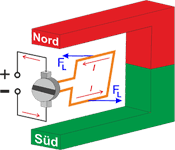
\includegraphics[width=4.3cm]{Bilder/elektromotor.png}\\
  {\scriptsize Elektromotor: Leiterschlaufe im Feld, $F$ dreht sie.}
\end{minipage}\hfill
\begin{minipage}[t]{7.5cm}\centering
  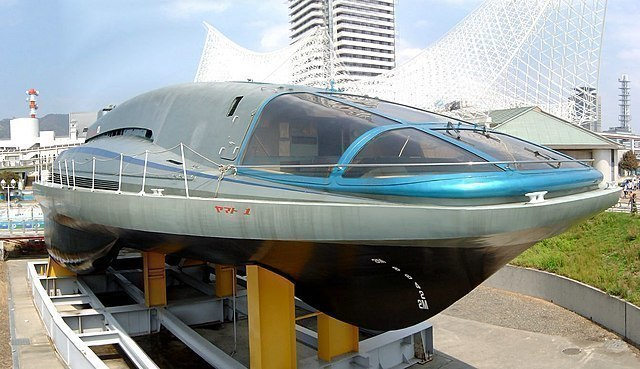
\includegraphics[width=7cm]{Bilder/mhd-ship-yamato-1.jpg}\\
  {\scriptsize MHD-Antrieb: die Yamato~1, angetrieben durch magnetische
  Kraft auf das leitfähige Meerwasser.}
\end{minipage}
\end{center}
Beim \textbf{Polarlicht} treffen geladene Teilchen aus dem Sonnenwind auf
das Erdmagnetfeld und werden auf gekrümmte Bahnen zu den Polen abgelenkt.
Beide Phänomene beruhen auf derselben Kraft: einmal wirkt sie auf einen
ganzen Leiter (die \textbf{\emph{magnetische Kraft}}), einmal auf eine
einzelne freie Ladung (die \textbf{\emph{Lorentzkraft}}). Genau diese
gekrümmte Bahn einzelner Ladungen nutzen Forscher auch gezielt: Im
\textbf{LHC} am CERN halten riesige Magnete Protonen auf einer 27\,km
langen Kreisbahn. Genau diese beiden Kräfte untersuchen Sie jetzt an drei
Experimenten.
\begin{center}
\begin{minipage}[t]{6cm}\centering
  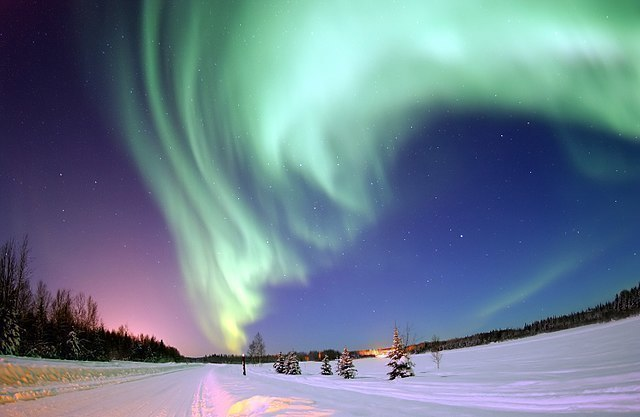
\includegraphics[width=6cm]{Bilder/aurora-borealis.jpg}\\
  {\scriptsize Polarlicht (Aurora borealis).}
\end{minipage}\hfill
\begin{minipage}[t]{7cm}\centering
  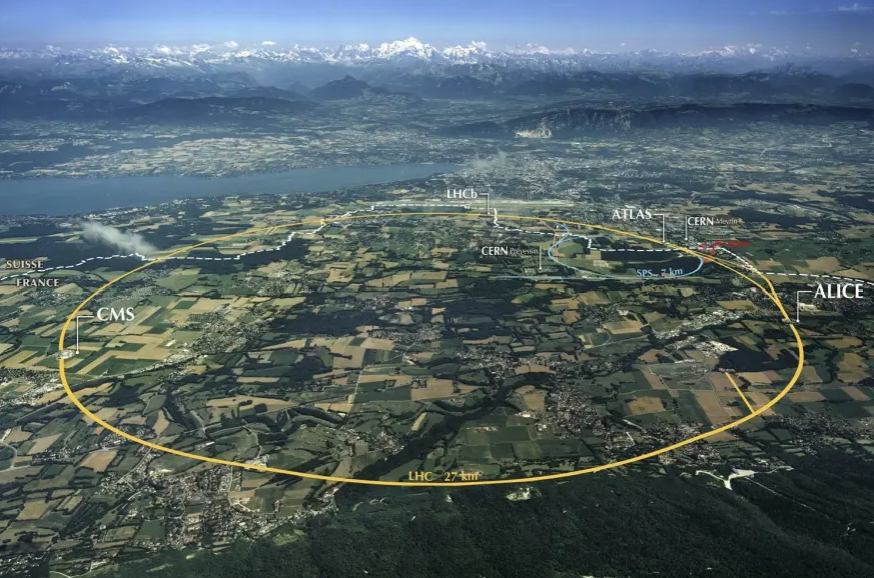
\includegraphics[width=7cm]{Bilder/LHC.png}\\
  {\scriptsize Der LHC-Ring (27\,km) bei Genf, mit seinen vier grossen
  Detektoren.}
\end{minipage}
\end{center}
\end{beispielbox}

% =============================================================================
% Experiment 1: Leiterschaukel (Partnerarbeit, LZ1)
% =============================================================================
\begin{questions}
\begin{groupbox}[Experiment 1 (Partnerarbeit): Leiterschaukel]
\question[3] Sie erhalten einen Aufbau mit einem Hufeisenmagneten und einem
lose aufgehängten, schaukelförmigen Leiter, der sich zwischen den Polen
befindet. Der Stromkreis lässt sich einschalten und umpolen.
\begin{center}
  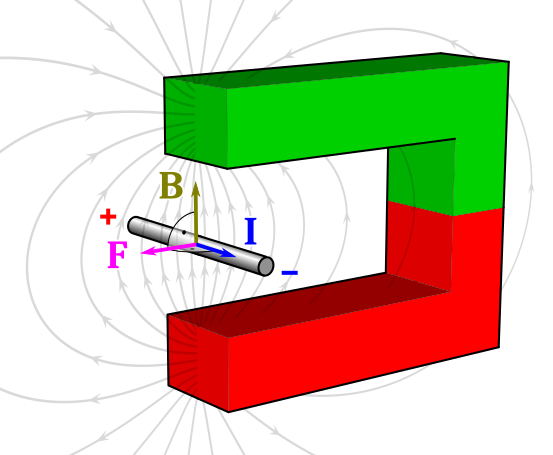
\includegraphics[width=6.5cm]{Bilder/leiterschaukel-experiment-preview.pdf}
\end{center}
{\scriptsize Leiterschaukel im Feld eines Hufeisenmagneten: Stromrichtung
$I$, Feldrichtung $B$, resultierende Kraft $F$ auf den Leiter.}
Schalten Sie den Strom ein und beobachten Sie, in welche Richtung sich die
Schaukel bewegt. Polen Sie anschliessend zuerst nur den Strom, dann zusätzlich
noch den Magneten um. Notieren Sie für alle drei Fälle, was Sie beobachten
(\textbf{noch ohne Erklärung}, nur die reine Beobachtung).
\Antwortraum{3}
\begin{solution}
Bei der ersten Polung schlägt die Schaukel in eine bestimmte Richtung aus.
Polen Sie \emph{nur} den Strom um, schlägt sie in die \emph{entgegengesetzte}
Richtung aus. Polen Sie zusätzlich auch noch den Magneten um (also beide
Male), schlägt sie wieder in die \emph{ursprüngliche} Richtung aus wie beim
ersten Versuch: Die Auslenkungsrichtung hängt also von \emph{beiden}
Polungen zusammen ab, nicht von einer allein.
\end{solution}
\end{groupbox}
\end{questions}

% =============================================================================
% Theorie: Magnetische Kraft F=IlB (allgemein + Spezialfall) und
% Drei-Finger-Regel (LZ2, LZ3)
% =============================================================================
\begin{theoriebox}[Die magnetische Kraft auf einen Leiter]
Ein stromdurchflossener Leiter (Länge $l$, Strom $I$) kann sich in einem
\textbf{\emph{externen}} Magnetfeld $B$ befinden, also einem Feld, das
\emph{nicht} vom Strom im Leiter selbst erzeugt wird, sondern von aussen
kommt (z.\,B. von einem Permanentmagneten oder einem anderen Leiter). Ein
solcher Leiter erfährt dann die \textbf{\emph{magnetische Kraft}}:
\begin{formelbox}[Magnetische Kraft]
\[
  \vec F = I\,\vec l\times\vec B, \qquad F = I\cdot l\cdot B\cdot\sin\alpha
\]
Einheit von $F$: $\si{\newton}$. $\alpha$ ist der Winkel zwischen der
Stromrichtung $\vec l$ und der Feldrichtung $\vec B$ (mit dem aus der
Mathematik bereits bekannten Kreuzprodukt).

\textbf{Spezialfall (senkrechtes Feld):} Steht der Leiter senkrecht zum
Feld ($\vec I\perp\vec B$, also $\alpha=90^\circ$), gilt $\sin\alpha=1$ und
damit einfach
\[
  F = I\cdot l\cdot B
\]
\end{formelbox}
\begin{center}
  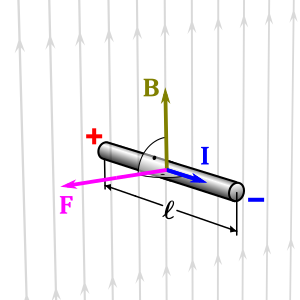
\includegraphics[width=6cm]{Bilder/magnetic-force-wire.pdf}
\end{center}
{\scriptsize Stromdurchflossenes Leiterstück der Länge $l$ im Feld $B$:
die magnetische Kraft $F$ steht senkrecht zu beiden.}

Die \textbf{\emph{Richtung}} dieser Kraft bestimmen Sie mit der
\textbf{\emph{Drei-Finger-Regel der rechten Hand}}: Daumen, Zeigefinger und
Mittelfinger stehen dabei paarweise senkrecht aufeinander.
\begin{center}
  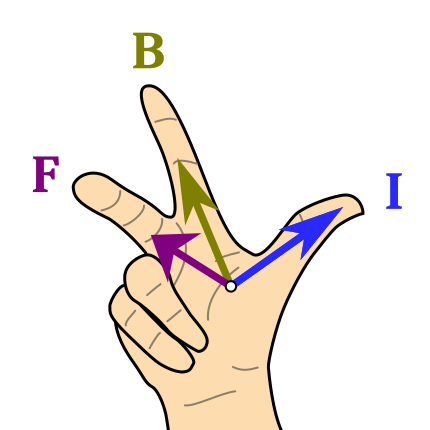
\includegraphics[width=5.5cm]{Bilder/uvw-regel-strom.pdf}
\end{center}
{\scriptsize Daumen = Stromrichtung $I$ (Ursache), Zeigefinger =
Feldrichtung $B$ (Vermittler), Mittelfinger = Kraftrichtung $F$ (Wirkung).
Rechte Hand, da $I$ per Konvention die Bewegungsrichtung positiver
Ladungsträger angibt.}
\end{theoriebox}

% =============================================================================
% Rückkehr: Leiterschaukel selbst erklären (LZ4)
% =============================================================================
\begin{questions}
\begin{taskbox}[Rückkehr: Erklären Sie Ihre eigene Beobachtung]
\question[8] Bearbeiten Sie diese Aufgabe zuerst \textbf{allein}, vergleichen
Sie danach \textbf{zu zweit} Ihre Antwort.

Bei Vektoren, die senkrecht zur Zeichenebene stehen, gilt folgende
Konvention: $\odot$ bedeutet, der Vektor zeigt aus der Ebene heraus, auf
Sie zu (wie die Spitze eines Pfeils, der Ihnen entgegenfliegt); $\otimes$
bedeutet, er zeigt in die Ebene hinein, von Ihnen weg (wie die Federn
eines Pfeils, der sich von Ihnen entfernt).

Die Skizze unten zeigt Ihren Aufbau von der Seite, entlang des
Leiterstabs geschaut: Der Nordpol liegt \textbf{unten}, der Südpol
\textbf{oben} (wie beim Foto in Experiment 1), der Leiterstab hängt im
Luftspalt zwischen den beiden Polen. Bei der ersten Polung aus Ihrer
Beobachtung von oben schwingt die Schaukel \textbf{nach rechts}.
\begin{parts}
  \part[4] Zeichnen Sie \textbf{alle drei} Vektoren direkt in die Skizze
  ein: die Feldrichtung $B$ (aus der Polbezeichnung), die Kraftrichtung
  $F$ (als Pfeil nach links oder rechts, passend zur obigen Beobachtung)
  und (mithilfe der Drei-Finger-Regel) die Stromrichtung $I$ im
  Leiterstab (mit dem passenden Symbol $\odot$/$\otimes$, da der
  Leiterstab hier im Querschnitt zu sehen ist).
  \begin{center}
  \begin{tikzpicture}[>=Latex,scale=1.1]
    \filldraw[fill=gray!25,draw=black,thick] (-1.3,0.9) rectangle (1.3,1.7);
    \node[font=\bfseries\Large] at (0,1.3) {S};
    \filldraw[fill=gray!25,draw=black,thick] (-1.3,-1.7) rectangle (1.3,-0.9);
    \node[font=\bfseries\Large] at (0,-1.3) {N};
    \draw[thick] (0,0) circle (0.18);
    \node[align=center,font=\scriptsize] at (0,-2.2) {Leiterstab\\(Querschnitt)};
  \end{tikzpicture}
  \end{center}
  \begin{solution}
  Die Feldrichtung $B$ zeigt vom Nordpol zum Südpol, hier also von unten
  nach oben. Die Beobachtung (Schaukel schwingt nach rechts) entspricht
  $F$ nach \textbf{rechts}. Mit der Drei-Finger-Regel (Daumen $I$,
  Zeigefinger $B$, Mittelfinger $F$) muss der Daumen dafür \textbf{in die
  Ebene hinein} zeigen: Der Strom fliesst im Leiterstab also \textbf{von
  Ihnen weg}, $I=\otimes$.
  \begin{center}
  \begin{tikzpicture}[>=Latex,scale=1.1]
    \filldraw[fill=gray!25,draw=black,thick] (-1.3,0.9) rectangle (1.3,1.7);
    \node[font=\bfseries\Large] at (0,1.3) {S};
    \filldraw[fill=gray!25,draw=black,thick] (-1.3,-1.7) rectangle (1.3,-0.9);
    \node[font=\bfseries\Large] at (0,-1.3) {N};
    \draw[thick,-{Latex[length=3mm]},blue] (-0.5,-0.7) -- (-0.5,0.7) node[pos=0.15,left,font=\scriptsize,black]{$B$};
    \node[font=\Large] at (0,0) {$\otimes$};
    \draw[thick,-{Latex[length=3mm]},red] (0.35,0) -- (1.5,0) node[midway,above,font=\scriptsize,black]{$F$};
    \node[align=center,font=\scriptsize] at (0,-2.2) {Leiterstab\\(Querschnitt)};
  \end{tikzpicture}
  \end{center}
  \end{solution}
  \part[2] Was ändert sich, wenn Sie \textbf{nur} den Strom umpolen (die
  Stromrichtung im Leiterstab kehrt sich also um), das Magnetfeld aber
  unverändert bleibt? Zeichnen Sie die neue Stromrichtung und die daraus
  resultierende Kraftrichtung in die zweite Skizze ein und geben Sie an,
  wohin die Schaukel jetzt schwingt.
  \begin{center}
  \begin{tikzpicture}[>=Latex,scale=1.1]
    \filldraw[fill=gray!25,draw=black,thick] (-1.3,0.9) rectangle (1.3,1.7);
    \node[font=\bfseries\Large] at (0,1.3) {S};
    \filldraw[fill=gray!25,draw=black,thick] (-1.3,-1.7) rectangle (1.3,-0.9);
    \node[font=\bfseries\Large] at (0,-1.3) {N};
    \draw[thick] (0,0) circle (0.18);
    \node[align=center,font=\scriptsize] at (0,-2.2) {Leiterstab\\(Querschnitt)};
  \end{tikzpicture}
  \end{center}
  \begin{solution}
  Die Feldrichtung $B$ bleibt unverändert (unten nach oben), der Strom
  fliesst jetzt aber umgekehrt, also \textbf{aus der Ebene heraus},
  $I=\odot$. Mit der Drei-Finger-Regel (Daumen $I$, Zeigefinger $B$,
  Mittelfinger $F$) zeigt der Mittelfinger jetzt \textbf{nach links}: Die
  Schaukel schwingt jetzt \textbf{nach links}, statt nach rechts.
  \begin{center}
  \begin{tikzpicture}[>=Latex,scale=1.1]
    \filldraw[fill=gray!25,draw=black,thick] (-1.3,0.9) rectangle (1.3,1.7);
    \node[font=\bfseries\Large] at (0,1.3) {S};
    \filldraw[fill=gray!25,draw=black,thick] (-1.3,-1.7) rectangle (1.3,-0.9);
    \node[font=\bfseries\Large] at (0,-1.3) {N};
    \draw[thick,-{Latex[length=3mm]},blue] (0.5,-0.7) -- (0.5,0.7) node[pos=0.15,right,font=\scriptsize,black]{$B$};
    \node[font=\Large] at (0,0) {$\odot$};
    \draw[thick,-{Latex[length=3mm]},red] (-0.35,0) -- (-1.5,0) node[midway,above,font=\scriptsize,black]{$F$};
    \node[align=center,font=\scriptsize] at (0,-2.2) {Leiterstab\\(Querschnitt)};
  \end{tikzpicture}
  \end{center}
  \end{solution}
  \part[2] Was ändert sich, wenn Sie stattdessen (ausgehend von der
  ursprünglichen Stromrichtung aus (a), also $I=\otimes$) \textbf{nur} den
  Magneten umdrehen (Nord- und Südpol vertauschen sich also), der Strom
  aber unverändert in dieselbe Richtung fliesst wie in (a)? Begründen Sie
  Ihre Antwort mit der Drei-Finger-Regel.
  \Antwortraum{2}
  \begin{solution}
  Jetzt zeigt $B$ von oben nach unten, während $I$ unverändert in die
  Ebene hinein zeigt ($I=\otimes$, wie in (a)). Die Drei-Finger-Regel
  liefert damit die entgegengesetzte Kraftrichtung: Die Schaukel schwingt
  jetzt \textbf{nach links}, statt nach rechts, genau wie bereits am
  Aufbau selbst
  beobachtet.
  \end{solution}
\end{parts}
\end{taskbox}
\end{questions}

% =============================================================================
% Experiment 2 (neu): Rollender Leiterstab auf der Schiene (Lehrer-Demo, LZ1)
% =============================================================================
\begin{questions}
\begin{taskbox}[Experiment 2 (Lehrerdemonstration): Rollender Leiterstab auf der Schiene]
\question[4] Die Lehrperson zeigt einen Leiterstab, der quer über zwei
parallele Schienen zwischen den Polen eines Magneten liegt und frei rollen
kann. Die Schienen sind an eine Stromquelle angeschlossen; die Skizze
zeigt den Aufbau von oben, mit der bekannten Stromrichtung $I$ im Stab und
der Feldrichtung $B$ des Magneten (Symbole wie oben: $\odot$/$\otimes$ =
senkrecht zur Zeichenebene).
\begin{center}
\begin{tikzpicture}[>=Latex,scale=1.0]
  \draw[very thick] (-3.5,1) -- (3,1);
  \draw[very thick] (-3.5,-1) -- (3,-1);
  \draw[thick] (-3.5,1) -- (-3.5,0.3);
  \draw[thick] (-3.5,-1) -- (-3.5,-0.3);
  \draw[thick] (-3.7,0.3) -- (-3.3,0.3);
  \draw[thick] (-3.6,-0.3) -- (-3.4,-0.3);
  \node[font=\scriptsize] at (-4.3,0) {Batterie};
  \draw[dashed,gray] (-1.5,-1.4) rectangle (1.5,1.4);
  \foreach \x in {-1,-0.3,0.4,1.1}{
    \foreach \y in {-0.9,-0.2,0.5}{
      \node[font=\small,gray] at (\x,\y) {$\otimes$};
    }
  }
  \node[font=\scriptsize,align=center] at (0,1.8) {Magnetfeld $B$\\(in die Tischebene hinein)};
  \draw[very thick,red] (0,1) -- (0,-1);
  \draw[thick,-{Latex[length=3mm]},red] (0,0.7) -- (0,0.1);
  \node[font=\scriptsize,black] at (0.35,0.85) {$I$};
  \node[align=center,font=\scriptsize] at (0,-1.9) {Leiterstab (Draufsicht,\\rollt auf den Schienen)};
\end{tikzpicture}
\end{center}
Sobald der Strom eingeschaltet wird, rollt der Stab die Schiene entlang
nach vorne (in der Skizze also nach rechts).
\begin{parts}
  \part[3] Zeichnen Sie mit der Drei-Finger-Regel die Kraftrichtung $F$
  auf den Stab direkt in die Skizze ein und bestätigen Sie damit, dass der
  Stab tatsächlich nach rechts rollen muss.
  \Antwortraum{3}
  \begin{solution}
  Daumen $I$ nach unten, Zeigefinger $B$ in die Ebene hinein: Der
  Mittelfinger $F$ zeigt dann nach rechts, in Richtung der Schienen. Das
  bestätigt die beobachtete Rollrichtung.
  \begin{center}
  \begin{tikzpicture}[>=Latex,scale=1.0]
    \draw[very thick] (-3.5,1) -- (3,1);
    \draw[very thick] (-3.5,-1) -- (3,-1);
    \draw[dashed,gray] (-1.5,-1.4) rectangle (1.5,1.4);
    \foreach \x in {-1,-0.3,0.4,1.1}{
      \foreach \y in {-0.9,-0.2,0.5}{
        \node[font=\small,gray] at (\x,\y) {$\otimes$};
      }
    }
    \draw[very thick,red] (0,1) -- (0,-1);
    \draw[thick,-{Latex[length=3mm]},red] (0,0.7) -- (0,0.1);
    \node[font=\scriptsize,black] at (0.35,0.85) {$I$};
    \draw[thick,-{Latex[length=3mm]},blue] (0,0) -- (1.8,0) node[midway,above,font=\scriptsize,black]{$F$};
  \end{tikzpicture}
  \end{center}
  \end{solution}
  \part[1] Nennen Sie ein alltägliches Gerät, das auf genau demselben
  Prinzip beruht.
  \Antwortraum{1}
  \begin{solution}
  Genau dieses Prinzip (Kraft auf einen stromdurchflossenen Leiter im
  Magnetfeld) treibt jeden \textbf{Elektromotor} an (siehe Einleitung).
  \end{solution}
\end{parts}
\end{taskbox}
\end{questions}

% =============================================================================
% Experiment 3: Zwei parallele Leiter (Lehrer-Demonstration, LZ1)
% =============================================================================
\begin{taskbox}[Experiment 3 (Lehrerdemonstration): Zwei parallele Leiter]
Die Lehrperson zeigt im Plenum zwei parallel hängende, stromdurchflossene
Drähte, deren Stromrichtung sich unabhängig voneinander umpolen lässt: Bei
\textbf{gleichgerichteten} Strömen ziehen sich die Drähte an, bei
\textbf{entgegengesetzt} gerichteten Strömen stossen sie sich ab.
\end{taskbox}

\begin{beispielbox}[Bereits bekannt und ein Stück Geschichte]
Sie kennen aus der Doppellektion zu Magnetfeldern bereits das Feld eines
geraden, stromdurchflossenen Leiters:
\[
  B = \frac{\mu_0}{2\pi}\cdot\frac{I}{r}
\]
Genau dieser Aufbau (zwei parallele, stromdurchflossene Leiter) diente
vor der SI-Neudefinition 2019 direkt zur \textbf{\emph{Definition}} der
Einheit Ampere: Über die gemessene Kraft zwischen zwei Leitern mit
bekanntem Abstand liess sich die Stromstärke festlegen, für die diese Kraft
gerade einen bestimmten Wert annimmt.
\end{beispielbox}

% =============================================================================
% Aufgabe: Ampere'sches Kraftgesetz herleiten + Anziehung/Abstossung (LZ7, LZ8)
% =============================================================================
\begin{questions}
\begin{taskbox}[Aufgabe: Kraft zwischen den beiden Leitern]
\question Kombinieren Sie Ihr Wissen über das Feld des geraden Leiters
($B=\frac{\mu_0}{2\pi}\cdot\frac{I}{r}$) mit der magnetischen Kraft
$F=I\cdot l\cdot B$ von oben, um die Kraft zwischen den beiden Leitern von
oben herzuleiten und ihre Richtung zu begründen.
\begin{parts}
  \part[3] Leiten Sie eine Formel für die Kraft \emph{pro Leiterlänge}
  $\frac{F}{l}$ zwischen zwei parallelen Leitern (Ströme $I_1$, $I_2$,
  Abstand $r$) her.
  \Antwortraum{4}
  \begin{solution}
  Das Feld des einen Leiters am Ort des anderen (Abstand $r$) ist
  \[
    B_1(r) = \frac{\mu_0}{2\pi}\cdot\frac{I_1}{r}
  \]
  Dieses Feld $B_1$ übt auf den zweiten Leiter (Strom $I_2$, Länge $l$) die
  magnetische Kraft aus:
  \[
    F = I_2\cdot l\cdot B_1
  \]
  Setzen wir $B_1(r)$ ein:
  \[
    F = I_2\cdot l\cdot\frac{\mu_0}{2\pi}\cdot\frac{I_1}{r}
  \]
  Umgestellt nach der Kraft \emph{pro Leiterlänge} $\frac{F}{l}$ ergibt sich
  das \textbf{\emph{Ampère'sche Kraftgesetz}}:
  \[
    \frac{F}{l} = \frac{\mu_0}{2\pi}\cdot\frac{I_1\cdot I_2}{r}, \qquad
    \text{Einheit von }\frac{F}{l}\colon\ \si{\newton\per\meter}
  \]
  \end{solution}
  \part[5] Für die \textbf{Richtung} betrachten Sie das Feld $B_1$, das der
  untere Leiter am Ort des oberen erzeugt: Zeichnen Sie dafür zuerst mit
  der \textbf{rechten Handregel} (Daumen in Stromrichtung, gekrümmte
  Finger zeigen die Feldrichtung) den Vektor $B_1$ am Ort des oberen
  Leiters in die beiden Skizzen unten ein. Bestimmen Sie anschliessend mit
  der \textbf{Drei-Finger-Regel} die Kraft $F_2$, die dieses Feld auf den
  oberen (stromdurchflossenen) Leiter ausübt, und zwar für \textbf{beide} Fälle.
  Erklären Sie damit, weshalb sich die Leiter bei gleichgerichteten
  Strömen anziehen und bei entgegengesetzten abstossen.
  \begin{center}
  \begin{minipage}[t]{7cm}\centering
    \begin{tikzpicture}[>=Latex,scale=1.2]
      \node[font=\Large] at (0,0) {$\odot$};
      \node[below=1pt,font=\scriptsize] at (0,-0.4) {$I_1$};
      \node[font=\Large] at (0,2.4) {$\otimes$};
      \node[above=1pt,font=\scriptsize] at (0,2.8) {$I_2$};
      \draw[<->] (0.9,0) -- (0.9,2.4) node[midway,right,font=\scriptsize]{$r$};
    \end{tikzpicture}\\
    {\scriptsize (a) entgegengesetzte Ströme}
  \end{minipage}\hfill
  \begin{minipage}[t]{7cm}\centering
    \begin{tikzpicture}[>=Latex,scale=1.2]
      \node[font=\Large] at (0,0) {$\odot$};
      \node[below=1pt,font=\scriptsize] at (0,-0.4) {$I_1$};
      \node[font=\Large] at (0,2.4) {$\odot$};
      \node[above=1pt,font=\scriptsize] at (0,2.8) {$I_2$};
      \draw[<->] (0.9,0) -- (0.9,2.4) node[midway,right,font=\scriptsize]{$r$};
    \end{tikzpicture}\\
    {\scriptsize (b) gleichgerichtete Ströme}
  \end{minipage}
  \end{center}
  {\scriptsize Symbole wie oben: $\odot$ = Strom aus der Ebene heraus, auf
  Sie zu; $\otimes$ = Strom in die Ebene hinein, von Ihnen weg.}
  \Antwortraum{5}
  \begin{solution}
  In beiden Fällen fliesst $I_1$ aus der Ebene heraus. Nach der rechten
  Handregel (Daumen aus der Ebene heraus, Finger krümmen sich gegen den
  Uhrzeigersinn) zeigt $B_1$ am Ort des oberen Leiters (direkt über
  $I_1$) deshalb in \textbf{beiden} Fällen nach \textbf{links}. Nach
  demselben Muster liefert $B_2$ (das Feld von $I_2$ am Ort des unteren
  Leiters) die Feldrichtung dort. So lassen sich Feld \textbf{und} Kraft
  für \textbf{beide} Leiter bestimmen, nicht nur für den oberen:
  \begin{center}
  \begin{minipage}[t]{7cm}\centering
    \begin{tikzpicture}[>=Latex,scale=1.2]
      \node[font=\Large] at (0,0) {$\odot$};
      \node[below=1pt,font=\scriptsize] at (0,-0.4) {$I_1$};
      \node[font=\Large] at (0,2.4) {$\otimes$};
      \node[above=1pt,font=\scriptsize] at (0,2.8) {$I_2$};
      \draw[thick,-{Latex[length=3mm]},blue] (-0.4,2.4) -- (-1.8,2.4) node[midway,above,font=\scriptsize,black]{$B_1$};
      \draw[thick,-{Latex[length=3mm]},red] (0.3,2.4) -- (0.3,3.6) node[midway,right,font=\scriptsize,black]{$F_2$};
      \draw[thick,-{Latex[length=3mm]},blue] (-0.4,0) -- (-1.8,0) node[midway,above,font=\scriptsize,black]{$B_2$};
      \draw[thick,-{Latex[length=3mm]},red] (0.3,0) -- (0.3,-1.2) node[midway,right,font=\scriptsize,black]{$F_1$};
    \end{tikzpicture}\\
    {\scriptsize (a) $F_1$ und $F_2$ zeigen jeweils vom anderen Leiter
    weg: Abstossung.}
  \end{minipage}\hfill
  \begin{minipage}[t]{7cm}\centering
    \begin{tikzpicture}[>=Latex,scale=1.2]
      \node[font=\Large] at (0,0) {$\odot$};
      \node[below=1pt,font=\scriptsize] at (0,-0.4) {$I_1$};
      \node[font=\Large] at (0,2.4) {$\odot$};
      \node[above=1pt,font=\scriptsize] at (0,2.8) {$I_2$};
      \draw[thick,-{Latex[length=3mm]},blue] (-0.4,2.4) -- (-1.8,2.4) node[midway,above,font=\scriptsize,black]{$B_1$};
      \draw[thick,-{Latex[length=3mm]},red] (0.3,2.4) -- (0.3,1.2) node[midway,right,font=\scriptsize,black]{$F_2$};
      \draw[thick,-{Latex[length=3mm]},blue] (0.4,0) -- (1.8,0) node[midway,above,font=\scriptsize,black]{$B_2$};
      \draw[thick,-{Latex[length=3mm]},red] (-0.3,0) -- (-0.3,1.2) node[midway,left,font=\scriptsize,black]{$F_1$};
    \end{tikzpicture}\\
    {\scriptsize (b) $F_1$ und $F_2$ zeigen jeweils zum anderen Leiter
    hin: Anziehung.}
  \end{minipage}
  \end{center}
  Fall (a), entgegengesetzte Ströme: Daumen $I_2$ in die Ebene hinein,
  Zeigefinger $B_1$ nach links. Der Mittelfinger $F_2$ zeigt nach oben,
  \textbf{vom} unteren Leiter weg: \textbf{Abstossung}. Am unteren Leiter
  liefert dieselbe Überlegung mit $I_1$ und $B_2$ eine Kraft $F_1$ nach
  unten, ebenfalls \textbf{vom} oberen Leiter weg: auch hier
  \textbf{Abstossung}, wie es das Wechselwirkungsprinzip (actio =
  reactio) verlangt. Fall (b), gleichgerichtete Ströme: analog zeigt
  $F_2$ nach unten (\textbf{zum} unteren Leiter hin) und $F_1$ nach oben
  (\textbf{zum} oberen Leiter hin): beidseitig \textbf{Anziehung}.
  Achtung, Verwechslungsgefahr mit Polen/Ladungen: Dort gilt \glqq gleich
  stösst ab\grqq{}. Bei parallelen Strömen gilt das Gegenteil.
  \end{solution}
\end{parts}
\end{taskbox}
\end{questions}

% =============================================================================
% Theorie: Lorentzkraft (aus der bereits bekannten magnetischen Kraft
% hergeleitet -- siehe institutionen/UZH-Praktikum-I: Herleitungsrichtung
% wurde umgedreht, sodass man von F=IlB zur Lorentzkraft F=qvB kommt)
% =============================================================================
\begin{theoriebox}[Die Lorentzkraft auf eine einzelne Ladung]
Ein Strom ist eine Bewegung vieler einzelner Ladungsträger. Jeder einzelne
dieser bewegten Ladungsträger befindet sich ebenfalls im Magnetfeld $B$ und
erfährt deshalb (unabhängig davon, ob er sich gerade in einem Leiter
befindet oder frei ist) eine eigene Kraft auf eine \textbf{einzelne}
Ladung $q$ mit Geschwindigkeit $v$: die \textbf{\emph{Lorentzkraft}}.
\begin{center}
  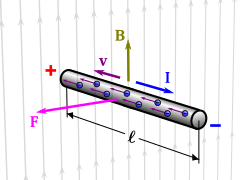
\includegraphics[width=6cm]{Bilder/magnetic-force-on-wire-with-electrons.pdf}
\end{center}
{\scriptsize Die einzelnen Ladungsträger im Leiter bewegen sich mit der
Driftgeschwindigkeit $v$ durch das Feld $B$ und erfahren je für sich eine
Kraft.}

Zeigen wir nun gemeinsam im Plenum, ausgehend von der bereits bekannten
magnetischen Kraft $F=IlB$ auf das ganze Leiterstück, welche Kraft davon
auf einen \textbf{einzelnen} Ladungsträger entfällt: die magnetische
Kraft ist nämlich nichts anderes als die Summe dieser Einzelkräfte über
alle Ladungsträger in einem Leiterstück, \emph{nicht} eine zweite,
unabhängige Kraft.

\ifprintanswers
\textbf{Herleitung:} Wir kennen bereits die magnetische Kraft auf ein
Leiterstück der Länge $l$:
\[
  F = I\cdot l\cdot B
\]
Nach der Definition der Stromstärke gilt $I=\frac{Q}{t}$, wobei $Q$ die
gesamte im Leiterstück enthaltene Ladung ist und $t$ die Zeit, die diese
Ladungsträger brauchen, um das Leiterstück zu durchqueren. Setzen wir
$I=\frac{Q}{t}$ direkt in die magnetische Kraft ein:
\[
  F = \frac{Q}{t}\cdot l\cdot B
\]
Umgestellt (den Bruch $\frac{Q}{t}$ mit $l$ zusammengefasst):
\[
  F = Q\cdot\frac{l}{t}\cdot B
\]
Die Ladungsträger bewegen sich mit der (mittleren) Driftgeschwindigkeit
$v$ durch das Leiterstück der Länge $l$ und benötigen dafür genau die
Zeit $t$, das heisst $\frac{l}{t}=v$. Setzen wir das ein:
\[
  F = Q\cdot v\cdot B
\]
Diese Kraft $F=QvB$ ist die \textbf{gesamte} Kraft auf \textbf{alle} $N$
Ladungsträger im Leiterstück zusammen, mit $Q=N\cdot q$ (jeder
Ladungsträger trägt dieselbe Ladung $q$). Da alle diese Ladungsträger
dieselbe Geschwindigkeit $v$ im selben Feld $B$ haben, entfällt auf
\textbf{jeden einzelnen} von ihnen der gleiche Anteil, den wir $F_N$
nennen (die Kraft auf eine von $N$ Ladungen):
\[
  F_N = \frac{F}{N} = \frac{Q\cdot v\cdot B}{N} = \frac{N\cdot q\cdot v\cdot B}{N}
\]
Kürzen von $N$ ergibt die Kraft auf eine einzelne Ladung:
\[
  F_N = q\cdot v\cdot B
\]
also genau die Lorentzkraft.
\else
\textbf{Platz für die gemeinsame Herleitung im Plenum:}
\Antwortraum{7}
\fi

Ausgeschrieben als Vektorgleichung lautet die Lorentzkraft:
\begin{formelbox}[Lorentzkraft]
\[
  \vec F = q\,\vec v\times\vec B, \qquad F = q\cdot v\cdot B\cdot\sin\alpha
\]
Einheit von $F$: $\si{\newton}$. $\alpha$ ist der Winkel zwischen der
Geschwindigkeit $\vec v$ und der Feldrichtung $\vec B$.

\textbf{Spezialfall (senkrechtes Feld):} Bei $\vec v\perp\vec B$ (also
$\alpha=90^\circ$) gilt wieder einfach
\[
  F = q\cdot v\cdot B
\]

Für die \textbf{Richtung} gilt weiterhin die Drei-Finger-Regel der
\textbf{rechten Hand}, jetzt mit dem Daumen in Richtung der
Ladungsgeschwindigkeit $v$ statt der Stromrichtung. Bei einer
\textbf{negativen} Ladung (z.\,B. einem Elektron) verwenden Sie
stattdessen die \textbf{\emph{technische Stromrichtung}}: Der Daumen
zeigt dann entgegen der tatsächlichen Bewegungsrichtung der Ladung, so
als würde sich eine positive Ladung in die Gegenrichtung bewegen. Sie
bleiben also immer bei der rechten Hand, ohne die Hand wechseln zu
müssen.
\begin{center}
  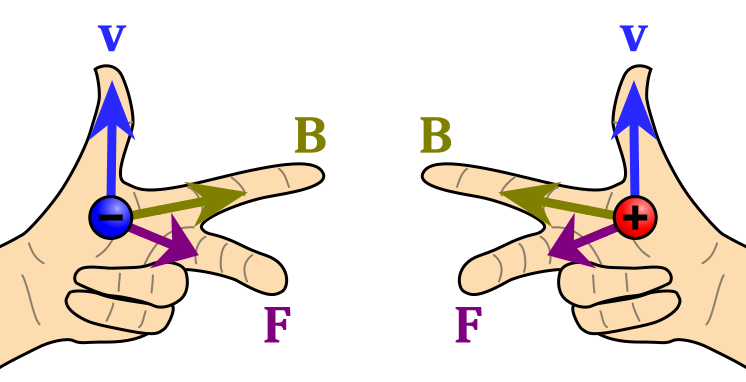
\includegraphics[width=8cm]{Bilder/uvw-regel-ladungen.pdf}
\end{center}
{\scriptsize Rechts: positive Ladung, rechte Hand, Daumen in Richtung
$v$. Links: einer negativen Ladung entspricht dieselbe rechte Hand, aber
mit dem Daumen in der technischen Stromrichtung (entgegen $v$). Genau
diese Variante verwenden wir immer, ohne auf die linke Hand zu wechseln.}
\end{formelbox}

Da die Lorentzkraft $F_L$ immer senkrecht zur Geschwindigkeit $v$ steht,
lenkt sie eine freie Ladung ständig zur Seite ab, ohne ihren Betrag zu
ändern. Was das für die Bewegung einer frei beweglichen Ladung bedeutet,
untersuchen Sie im separaten Fadenstrahlrohrdokument zu dieser
Doppellektion.
\end{theoriebox}

\end{document}
